% Le titre de la partie
\section{Diverses utilisation possibles}

%%%%%%%%%%%%%%%%%%%%%%%%%%%%%%%%%%%%%%%%%%%%%%%%
%%%%%%%%%%%%%%%%%%%%%%%%%%%%%%%%%%%%%%%%%%%%%%%%

\begin{frame}
	\frametitle{Un devoir par TP par élève}
	%\framesubtitle{}

	\begin{itemize}[<+->]
		\item Avantages:
			\begin{itemize}[<+->]
					\item Bien pour démarrer

					\item Pas d'action à faire sur le repository après avoir distribué le devoir

					\item Possibilité de corriger si les «béta-testeurs» trouvent des bugs: sera pris en compte pour les connexions ultérieures (mais pas pour ceux qui ont déjà accepté le devoir)
			\end{itemize}
		\item Inconvénients:
			\begin{itemize}[<+->]
					\item Accumulation de nombreux dossiers dans le répertoire \texttt{GitHub/}

					\item Nécessite de cliquer sur un lien à chaque nouveau TP (dur dur pour les élèves...)

					\item Demande de rappatrier systématiquement les dossiers par «classroom assistant» via l'interface web.
			\end{itemize}
	\end{itemize}

\end{frame}

%%%%%%%%%%%%%%%%%%%%%%%%%%%%%%%%%%%%%%%%%%%%%%%%
%%%%%%%%%%%%%%%%%%%%%%%%%%%%%%%%%%%%%%%%%%%%%%%%

\begin{frame}
	\frametitle{Un dossier semestriel par élève}
	%\framesubtitle{}

	\begin{itemize}[<+->]
		\item Avantages:
			\begin{itemize}[<+->]
				\item Possibilité d'organiser les dossiers (par TP, par PP, etc.)

				\item Un seul rappatriement global, puis des «pull» suffisent dans chaque dossier (scriptable)

				\item Les «pull» récupèrent en parallèles tous les projets en cours

				\item Ajouts automatisés des nouveaux dossiers, modifications des instructions possible par après
			\end{itemize}
		\item Inconvénients:
			\begin{itemize}[<+->]
				\item Nécessité de savoir scripter l'ajout automatique dans tous les dossiers
			\end{itemize}
	\end{itemize}

\end{frame}

%%%%%%%%%%%%%%%%%%%%%%%%%%%%%%%%%%%%%%%%%%%%%%%%
% Diapo exemple: le code informatique impose un
% environnement "fragile" pour la frame
%%%%%%%%%%%%%%%%%%%%%%%%%%%%%%%%%%%%%%%%%%%%%%%%

\begin{frame}[fragile]
	\frametitle{Exemples de script}
	\framesubtitle{«Pull» sur tous les repositories}

	\begin{code}
	\begin{minted}[linenos]{python}
base = "Info_sem2_2018-2019"
import glob,sys,os,subprocess
dossiers = glob.glob(base + '/' + base + '*')
racine = os.getcwd()
for d in sorted(dossiers):
    print("On s'occupe de {}".format(d))
    os.chdir(d)
    subprocess.call(['git','checkout','master'])
    subprocess.call(['git','pull'])
    os.chdir(racine)
	\end{minted}
	\end{code}
\end{frame}

%%%%%%%%%%%%%%%%%%%%%%%%%%%%%%%%%%%%%%%%%%%%%%%%
%%%%%%%%%%%%%%%%%%%%%%%%%%%%%%%%%%%%%%%%%%%%%%%%

\begin{frame}[fragile]
	\frametitle{Exemples de script}
	\framesubtitle{Ajout sur tous les repositories, partie 1}

	\begin{code}
	\begin{minted}[linenos]{python}
import glob,subprocess,os
base = "Info_sem2_2018-2019"
origin = '/chemin/vers/PP17'
target = 'PP/'
commit_message = "Arrivée du PP17"
dossiers = glob.glob(base + '/' + base + '*')
racine = os.getcwd()
	\end{minted}
	\end{code}
\end{frame}


%%%%%%%%%%%%%%%%%%%%%%%%%%%%%%%%%%%%%%%%%%%%%%%%
%%%%%%%%%%%%%%%%%%%%%%%%%%%%%%%%%%%%%%%%%%%%%%%%

\begin{frame}[fragile]
	\frametitle{Exemples de script}
	\framesubtitle{Ajout sur tous les repositories, partie 2}

	\begin{code}
	\begin{minted}[linenos]{python}
for d in sorted(dossiers):
    print("On s'occupe de {}".format(d))
    os.chdir(d)
    print('PULL')
    subprocess.call(['git','pull'])
    print('CP and COMMIT')
    subprocess.call(['cp','-R',origin,target])
    subprocess.call(['git','add','.'])
    subprocess.call(['git','commit','-m',commit_message])
    print('PUSH')
    subprocess.call(['git','push'])
    os.chdir(racine)
	\end{minted}
	\end{code}
\end{frame}


%%%%%%%%%%%%%%%%%%%%%%%%%%%%%%%%%%%%%%%%%%%%%%%%
%%%%%%%%%%%%%%%%%%%%%%%%%%%%%%%%%%%%%%%%%%%%%%%%

\begin{frame}
	\frametitle{Autres utilisations}
	\framesubtitle{Les TIPE}

	\begin{center}
		Voir \url{https://github.com/PCSIKleber/TIPE_2020}
	\end{center}

	\begin{itemize}[<+->]
		\item Travail en groupe

		\item Dossier commun (mieux pour suivre les versions des simulations informatiques)

		\item Travail en simultané via l'interface web
	\end{itemize}
\end{frame}

\begin{frame}
	\frametitle{Autres utilisations}
	\framesubtitle{Les TIPE}

	\begin{center}
		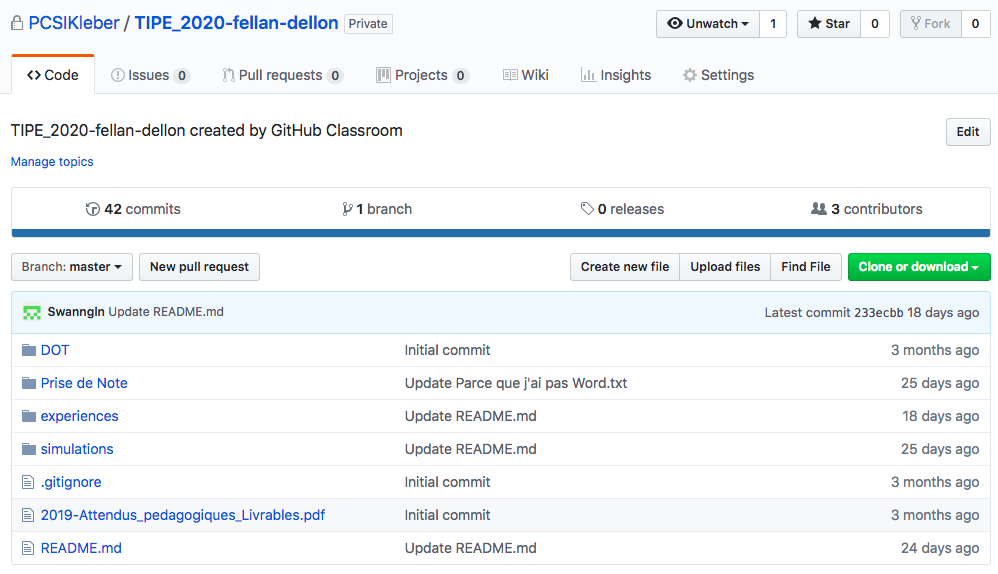
\includegraphics[width=\linewidth]{figures/TIPE1.png}
	\end{center}

\end{frame}

%%%%%%%%%%%%%%%%%%%%%%%%%%%%%%%%%%%%%%%%%%%%%%%%
%%%%%%%%%%%%%%%%%%%%%%%%%%%%%%%%%%%%%%%%%%%%%%%%

\begin{frame}
	\frametitle{Autres utilisations}
	\framesubtitle{Résumés de cours en \LaTeX}

	\begin{center}
		
\includegraphics[width=\linewidth]{figures/resumes_physique.png}
	\end{center}
	\begin{itemize}[<+->]
		\item Travail en groupe à l'échelle de la classe

		\item Travail en simultané via l'interface web (pour éviter les problèmes de fusion à gérer)

		\item Seul le prof a la main sur la génération du pdf via OverLeaf (beaucoup de boulot pour corriger les erreurs de syntaxe, mais le résultat est plutôt pas mal !)
	\end{itemize}
\end{frame}

%%%%%%%%%%%%%%%%%%%%%%%%%%%%%%%%%%%%%%%%%%%%%%%%
%%%%%%%%%%%%%%%%%%%%%%%%%%%%%%%%%%%%%%%%%%%%%%%%

\begin{frame}
	\frametitle{Autres utilisations}
	\framesubtitle{Boîte à outils pour TP de physique}

	\begin{center}
		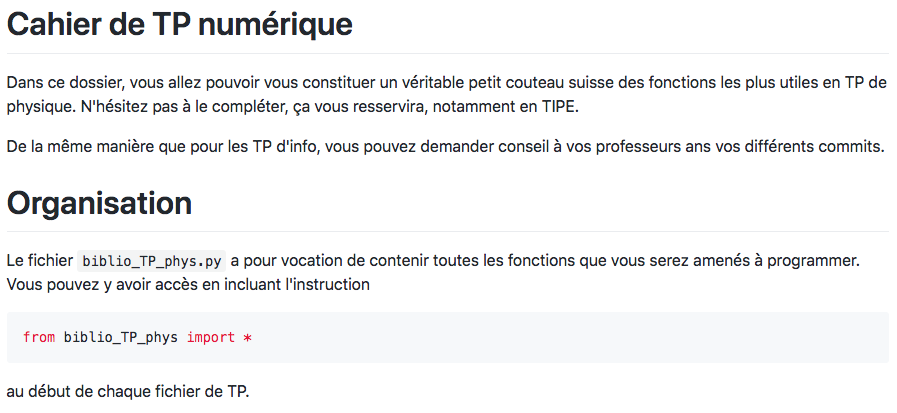
\includegraphics[width=\linewidth]{figures/cahier_de_TP.png}
	\end{center}
\end{frame}

\begin{frame}
	\frametitle{Autres utilisations}
	\framesubtitle{Boîte à outils pour TP de physique}


	\begin{itemize}[<+->]
		\item Travail en groupe (mais problème des binômes non stables)

		\item Permet de mettre en commun les mesures et scripts de traitement

		\item L'an prochain, dossier unique pour toute la classe avec des sous-dossiers par élève pour que tout le monde puisse accéder aux mesures de tout le monde (échange plus facile si les binômes changent)
	\end{itemize}
\end{frame}
